% !TeX TXS-program:compile = txs:///pdflatex/[--shell-escape]
% !TeX root = gnn-pres
% !TeX encoding = UTF-8
% !TeX spellcheck = en_US
% https://orcid.org/0000-0003-4586-8500


%\documentclass[14pt]{beamer}
\documentclass[aspectratio=169]{beamer} % Other possible values are: 1610, 149, 54, 43 and 32. By default, it is to 128mm by 96mm(4:3)

\documentclass{article}
\usepackage{blindtext}

%%% FONTS %%%
\usepackage[T1]{fontenc}
\usepackage[utf8]{inputenc}
\usepackage[english]{babel}
%\usepackage{tgpagella} % set the document font to TeX Gyre Pagella
%\usepackage{tgbonum} % set the document font to TeX Gyre Bonum
%\usepackage{fontawesome5} % The Creative Commons icons

%%% DRAFT watermark %%%
\usepackage{draftwatermark}
\SetWatermarkText{DRAFT}
\SetWatermarkScale{5.1}
\SetWatermarkLightness{0.8}

\usepackage{xcolor} % \textcolor{red}{text} will be red for notes
\definecolor{lightgray}{gray}{0.6}
\definecolor{medgray}{gray}{0.4}

\usepackage{hyperref}
\hypersetup{
	colorlinks=true,
	urlcolor= blue,
	citecolor=blue,
	linkcolor= blue,
	%bookmarks=true,
	%bookmarksopen=false,
}

% Code to add paragraph numbers and titles
\newif\ifptitle
\newif\ifpnumber
\newcounter{para}
\newcommand\ptitle[1]{\par\refstepcounter{para}
	{\ifpnumber{\noindent\textcolor{lightgray}{\textbf{\thepara}}\indent}\fi}
	{\ifptitle{\textbf{[{#1}]}}\fi}}
\ptitletrue  % comment this line to hide paragraph titles
\pnumbertrue  % comment this line to hide paragraph numbers

% for inserting images in line
\usepackage{graphicx}
\graphicspath{ {code/} }

%\usepackage[verbose]{wrapfig} % wrap text around image

\definecolor{myblue}{HTML}{4285F4} % color table cells

\usepackage[tablegrid]{vhistory} % version history package


% Allows to rewrite the same title in the supplement
\newcommand{\mytitle}{Analysis and Optimization of Security Infrastructure with Deep Learning Methods}
\usepackage{authblk}
\usepackage{comment} % allows block comments

\usepackage{ragged2e} % use flush and justify for text blocks
\usepackage{csquotes} % use \displayquote{} in the doc

%%% GRAPHICS  AND CODE BLOCKS %%%
\usepackage[listings, minted]{tcolorbox}
\usepackage{xcolor,colortbl}
\definecolor{myblue}{RGB}{0,163,243}
\definecolor{mygrey}{RGB}{128,128,128}
\definecolor{whitesmoke}{RGB}{245,245,245}
\newtcolorbox[auto counter, number within=section]{mybox}[2][]{
	colbacktitle=mygrey,
	colback=whitesmoke,
	title={#2},
	fonttitle=\ttfamily\small,
	fontupper=\sffamily\small,
	halign=flush left,
	rounded corners
}

% Headers and footers
\usepackage{fancyhdr}
\pagestyle{fancy}
\fancyhf{}
\lhead{\mytitle}
\lfoot{\tiny{November 20, 2021}}
\rfoot{\tiny{version: \vhCurrentVersion}}

\usepackage{glossaries}
	\makeglossaries

\newacronym{Edge}{Edge}{define edge}
\newacronym{GitOps}{GitOps}{Implementing  version control, collaboration, compliance, and CI/CD tooling for infrastructure automation}
\newacronym{Node}{Node}{define a node}
\newacronym{Scalar}{Scalar}{define a scalar here}
\newacronym{Vector}{Vector}{define a vector here}

\newcommand*{\myglossaryindent}{0.65cm}
\newcommand*{\myglsdescwidth}{10cm}



% Table of Contents at Section start
\AtBeginSection[]
{
    \begin{frame}
        \frametitle{\bfseries\Huge\textcolor{black}{.}}
        \tableofcontents[currentsection]
    \end{frame}
}

\begin{document}

%%% Title Slide %%%
\usebackgroundtemplate{
\includegraphics[width=\paperwidth]{../images/landscape.jpg}}
\begin{frame}
    \setlength{\TPHorizModule}{\textwidth}
    \setlength{\TPVertModule}{\textwidth}
    \begin{textblock}{0.6}(0.05,0.05)
      \bfseries\Huge\textcolor{cyan}{Learning About Deep Learning, and Maybe a Few Other Things}
    \end{textblock}
    % \begin{textblock}{WIDTH}(XCOORDINATE,YCOORDINATE)
    \begin{textblock}{0.5}(0.65,0.52)
        \bfseries\textcolor{green}{Franklin Diaz, Cosmic Voyager}
    \end{textblock}
\end{frame}

% Intro Section
\usebackgroundtemplate{
\includegraphics[width=\paperwidth]{../images/field.jpg}}
\section{Introduction}

\usebackgroundtemplate{
\includegraphics[width=\paperwidth]{../images/tree.jpg}}
\begin{frame}{}
    \setlength{\TPHorizModule}{\textwidth}
    \setlength{\TPVertModule}{\textwidth}
    % Slide title in upper left
    \begin{textblock}{0.74}(0.05,0.05)
        \bfseries\large\textcolor{white}{About Me}
    \end{textblock}

    \begin{columns}
        \begin{column}{0.5\textwidth}
            \begin{itemize}
                \item I am a Security Consultant at Palo Alto Networks, cloud and automation for past 2+ years
                \item Did Data Eng/DevSecOps at Salesforce for 5 years.
            \item Been going to security conferences for a while.
            \end{itemize}
        \end{column}
        \begin{column}{0.45\textwidth}
            \begin{center}
            
\includegraphics[width=1.0\linewidth, height=0.7\textheight]{../images/me.jpg}
            \end{center}
        \end{column}
    \end{columns}
\end{frame}

\usebackgroundtemplate{
\includegraphics[width=\paperwidth]{../images/tree.jpg}}
\begin{frame}{}
    \setlength{\TPHorizModule}{\textwidth}
    \setlength{\TPVertModule}{\textwidth}
    \begin{textblock}{0.74}(0.05,0.05)
        \bfseries\large\textcolor{white}{The Project}
    \end{textblock}

    \begin{columns} % \flushleft
        \begin{column}{0.8\textwidth}
            \begin{itemize}
                \item Realized that Terraform can output directed graphs.
                \item Had done a lot of work at Salesforce with DiGraphs, AirFlow, etc. so I was somewhat familiar with this type of data.
                \item What can we do with these directed graphs?
                \item Try to understand all these cool looking math symbols.
            \end{itemize}
        \end{column}
    \end{columns}
\end{frame}

\usebackgroundtemplate{
\includegraphics[width=\paperwidth]{../images/tree.jpg}}
\begin{frame}{}
    \setlength{\TPHorizModule}{\textwidth}
    \setlength{\TPVertModule}{\textwidth}
    % Slide title in upper left
    \begin{textblock}{0.74}(0.05,0.05)
        \bfseries\large\textcolor{white}{What's a DiGraph?}
    \end{textblock}

    \begin{columns}
        \begin{column}{0.5\textwidth}
            \begin{center}
                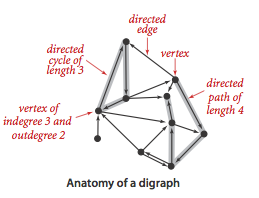
\includegraphics[width=1.0\linewidth,height=0.7\textheight]{../images/digraph-anatomy.png}
            \end{center}
         \end{column}
         \begin{column}{0.5\textwidth}
             \begin{center}
                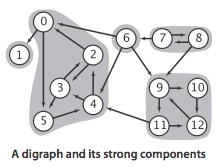
\includegraphics[width=1.0\linewidth,height=0.7\textheight]{../images/strong-components.png}
             \end{center}
        \end{column}
    \end{columns}
\end{frame}

\note[itemize]{
    \item The big takeaway here is the idea of ``edges'' and ``nodes''
    \item \href{https://algs4.cs.princeton.edu/42digraph/}{Source: Algorithms, 4th Edition, by Robert Sedgewick and Kevin Wayne}
    \item \href{https://www.youtube.com/watch?v=mXoiHgH4mEE}{Wrath of Math!}
}

\usebackgroundtemplate{
\includegraphics[width=\paperwidth]{../images/field.jpg}}
\section{What is Deep Learning, Exactly?}

\usebackgroundtemplate{
\includegraphics[width=\paperwidth]{../images/tree.jpg}}
\begin{frame}{}
    \setlength{\TPHorizModule}{\textwidth}
    \setlength{\TPVertModule}{\textwidth}
    % Slide title in upper left
    \begin{textblock}{0.74}(0.05,0.05)
        \bfseries\large\textcolor{white}{Quick Intro to a Giant Topic}
    \end{textblock}

    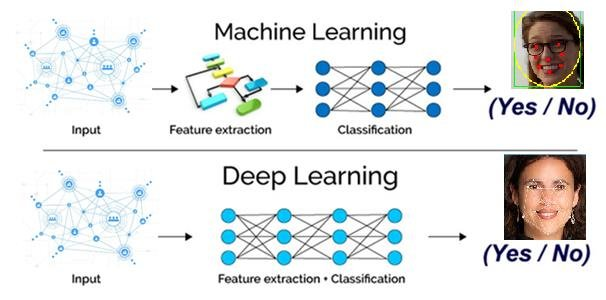
\includegraphics[width=1.0\linewidth,height=0.7\textheight]{../images/Diff-ML-DL.jpg}

\end{frame}

\note[itemize]{
    \item ML feature extraction can be a huge undertaking, up to 80\% of a project.
    \item DL attempts to automatically learn features that are most useful for a task from raw data.
    \item The nodes in a digraph are ``neurons'' or ``units'' in the DL/graph theory context.
    \item The neurons perform two steps. They calculate a ``weighted sum'' and pass the result through an ``activation function'' such as a rectifier activation function.
    \item These neurons or units that go through the rectifier function are called ``RelUs'' for short. Lot's of descriptive info in this one term!
    \item Depth of the GNN is measured by the number of connected layers.
    \item DL needs very large data sets for accurate feature determination. Data sets with lots of features are known as ``high density''.
}

\usebackgroundtemplate{
\includegraphics[width=\paperwidth]{../images/field.jpg}}
\section{The Journey}

\usebackgroundtemplate{
\includegraphics[width=\paperwidth]{../images/tree.jpg}}
\begin{frame}{}
    \setlength{\TPHorizModule}{\textwidth}
    \setlength{\TPVertModule}{\textwidth}
    % Slide title in upper left
    \begin{textblock}{0.74}(0.05,0.05)
        \bfseries\large\textcolor{white}{What Have I Gotten Myself Into?}
    \end{textblock}
    % main body bullet points
    \begin{itemize}
        \item This is an example of a list.
        \item Important business information.
    \end{itemize}
\end{frame}

\usebackgroundtemplate{
\includegraphics[width=\paperwidth]{../images/tree.jpg}}
\begin{frame}{}
    \setlength{\TPHorizModule}{\textwidth}
    \setlength{\TPVertModule}{\textwidth}
    % Slide title in upper left
    \begin{textblock}{0.74}(0.05,0.05)
        \bfseries\large\textcolor{white}{Yak Shaving, Side Quests, Endless Rabbit Holes}
    \end{textblock}
    % main body
    \begin{itemize}
        \item Makefiles and GNU Autotools
        \item NVIDA Jetson Nano as cluster nodes
        \item SLURM cluster scheduler
        \item OpenMPI for parallel builds
        \item Docker and Containers
        \item k8s and Rancher k3s
        \item Data Version Control \href{https://dvc.org}{dvc.org}
        \item Storing/accessing data in GCP buckets
        \item Continuous Machine Learning \href{https://cml.dev/}{cml.dev}
        \item Internal Pypi and Debian/Raspbian mirror (used too much bandwidth on home connection)
    \end{itemize}
\end{frame}

\defverbatim[colored]\lstI{
\begin{lstlisting}[language=Python,basicstyle=\ttfamily,keywordstyle=\color{red}]

# Generate a PNG from Terraform
terraform graph | dot -Tpng > graph.png

# Generate vector graphic from Terraform
terraform graph | dot -Tsvg -o graph.svg
    \end{lstlisting}
}

\usebackgroundtemplate{
\includegraphics[width=\paperwidth]{../images/tree.jpg}}
\begin{frame}{}
    \setlength{\TPHorizModule}{\textwidth}
    \setlength{\TPVertModule}{\textwidth}
    % Slide title in upper left
    \begin{textblock}{0.74}(0.05,0.05)
        \bfseries\large\textcolor{white}{Data Collection}
    \end{textblock}
    % main body
    A big barrier to entry was removed by the ability to output a Directed Graph from Terraform.
\lstI
\end{frame}

\usebackgroundtemplate{
\includegraphics[width=\paperwidth]{../images/field.jpg}}
\section{Visualizations}

\usebackgroundtemplate{
\includegraphics[width=\paperwidth]{../images/tree.jpg}}
\begin{frame}{}
    \setlength{\TPHorizModule}{\textwidth}
    \setlength{\TPVertModule}{\textwidth}
    % Slide title in upper left
    \begin{textblock}{0.74}(0.05,0.05)
        \bfseries\large\textcolor{white}{Graphviz/Dot output}
    \end{textblock}
    \begin{textblock}{0.75}(0.025,0.08)

    \begin{figure}
        \centering
        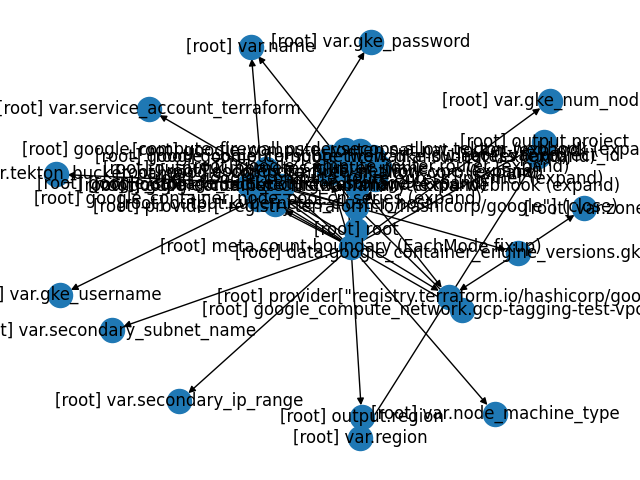
\includegraphics[width=1.0\linewidth, height=0.7\textheight]{../images/graph-dl-test}
        \caption{}
        \label{fig:graph-dl-test}
    \end{figure}

\end{textblock}
\end{frame}
\note[itemize]{
    \item This is the first thing I saw when first converting the data.
    \item Was excited here since I was able to change the color of the nodes.
    \item Obviously this is not yet a usable result.
}

\usebackgroundtemplate{
\includegraphics[width=\paperwidth]{../images/field.jpg}}
\section{Sources and Citations}

\usebackgroundtemplate{
\includegraphics[width=\paperwidth]{../images/tree.jpg}}
\begin{frame}{}
    \setlength{\TPHorizModule}{\textwidth}
    \setlength{\TPVertModule}{\textwidth}
    % Slide title in upper left
    \begin{textblock}{0.74}(0.05,0.05)
        \bfseries\large\textcolor{white}{Sources and Citations}
    \end{textblock}
    % main body bullet points
    \begin{itemize}
        \item This is an example of a list.
        \item Important business information.
    \end{itemize}
\end{frame}
\note[itemize]{
    \item point 1
    \item point 2
}

\end{document}
